\documentclass{article}
\usepackage{graphicx} % Required for inserting images

\title{Notes on ECG machines}
\author{Arsh Arora}
\date{May 2023}

\begin{document}

\maketitle

\section{Basics of Electrocardiograph}
The electrocardiograph (ECG) is an instrument, which records the electrical activity of the heart. ECG provides valuable information about a wide range of cardiac disorders such as the presence of an inactive part (infarction) or an enlargement (cardiac hypertrophy) of the heart muscle. Electrocardiographs are used in catheteriza-tion laboratories, coronary care units and for routine diagnostic applications in cardiology.
\subsection{Block Diagram of ECG}
\begin{center}
    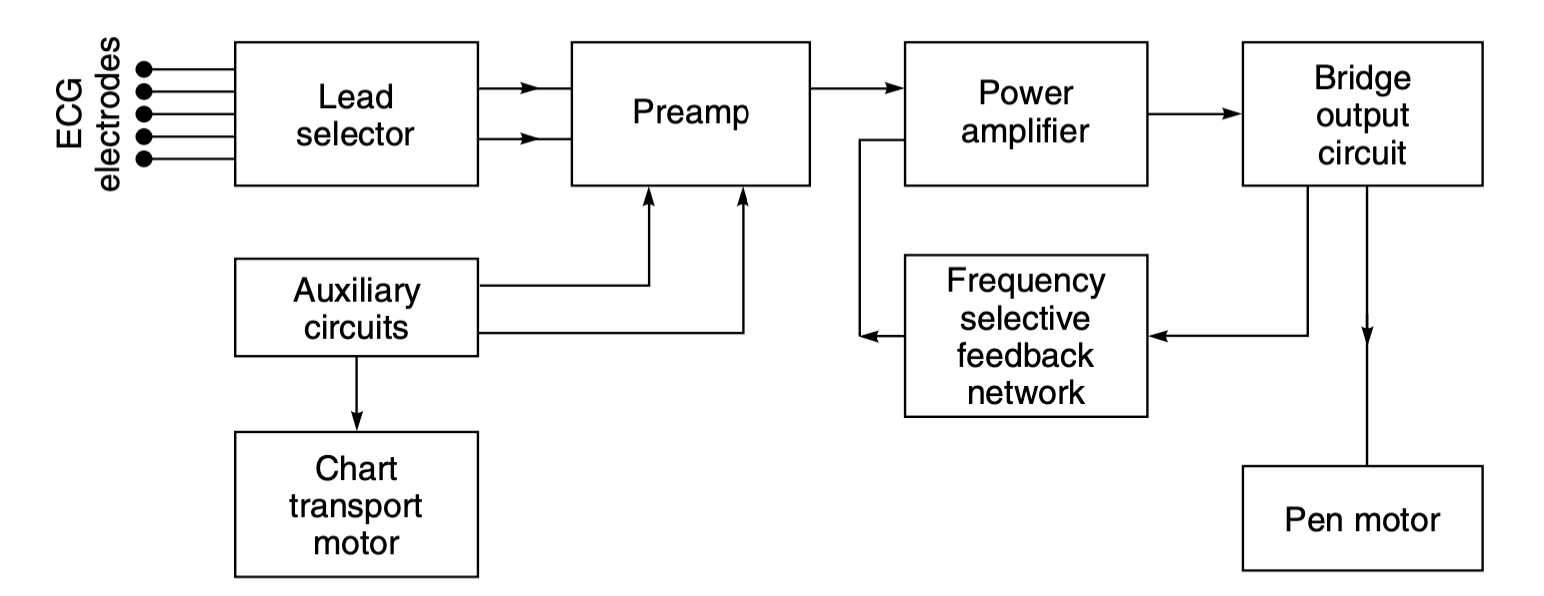
\includegraphics[scale=0.4]{Screenshot 2023-05-02 at 7.00.42 PM.png}
\end{center}
The potentials picked up by the patient electrodes are taken to the lead selector switch. In the lead selector, the electrodes are selected two by two according to the lead program. By means of capacitive coupling, the signal is connected symmetrically to the long-tail pair differential preamplifier. The preamplifier is usually a three or four stage differential amplifier having a sufficiently large negative current feedback, from the end stage to the first stage, which gives a stabilizing effect. The amplified output signal is picked up single-ended and is given to the power amplifier. The power amplifier is generally of the push-pull differential type. The base of one input transistor of this amplifier is driven by the preamplified unsymmetrical signal. The base of the other transistor is driven by the feedback signal resulting from the pen position and connected via frequency selective network. The output of the power amplifier is single-ended and is fed to the pen motor, which deflects the writing arm on the paper.\\
\subsubsection{Isolation of Pre-amplifier}
It is a traditional given for all electrocardiographs to have the RL connected to the chassis and then to the ground. This is a solid path for the earthing of any leakage current which would cause a serious electric hazard. To avoid this, as the micro shock hazard came to be understood at a better level, particularly when inter cardiac catheters are employed, the necessity to separate the subject from the ground was very actively emphasised. For this reason the patient leads would have to be isolated from the ground for all line operated units.\\
The basic diagram for a isolated pre-amplifier is as follows.
\begin{center}
    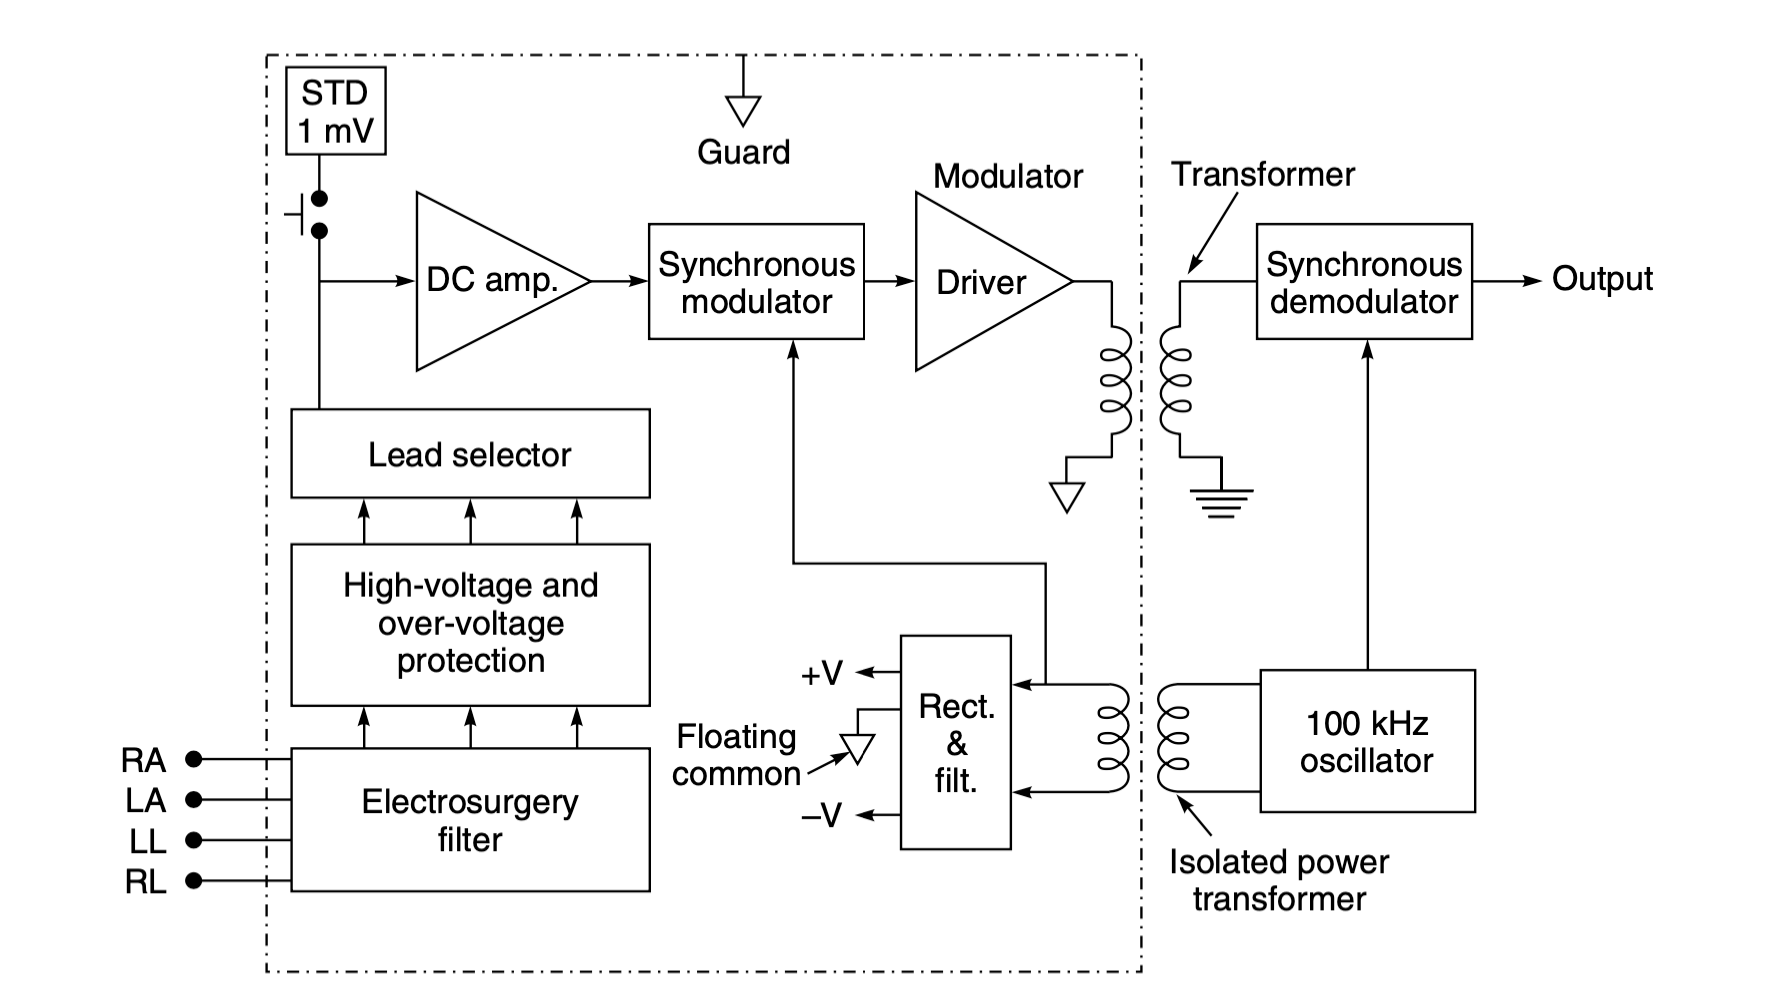
\includegraphics[scale=0.4]{Screenshot 2023-05-02 at 7.31.20 PM.png}
\end{center}
The price for this protection is extremely high as it brings out a lot of amplifier noise due to the high series resistance in each lead attached.\\
\\
Isolation of the patient preamplifier can also be obtained using an optical isolator. The high common-mode rejection of the amplifier is obtained by proper shielding. The effective capacitance from the input leads to the earth is made negligible. The preamplifier circuitry should is preferably be shielded in a separate case.\\
\\
To minimize the common-mode signal between the body of the patient and the floating ground, a right leg drive circuit is used. The common-mode signals after amplification in a preamplifier are inverted and fed back to the right leg electrode, reducing the common mode voltage on the input with respect to the floating ground.
\begin{center}
    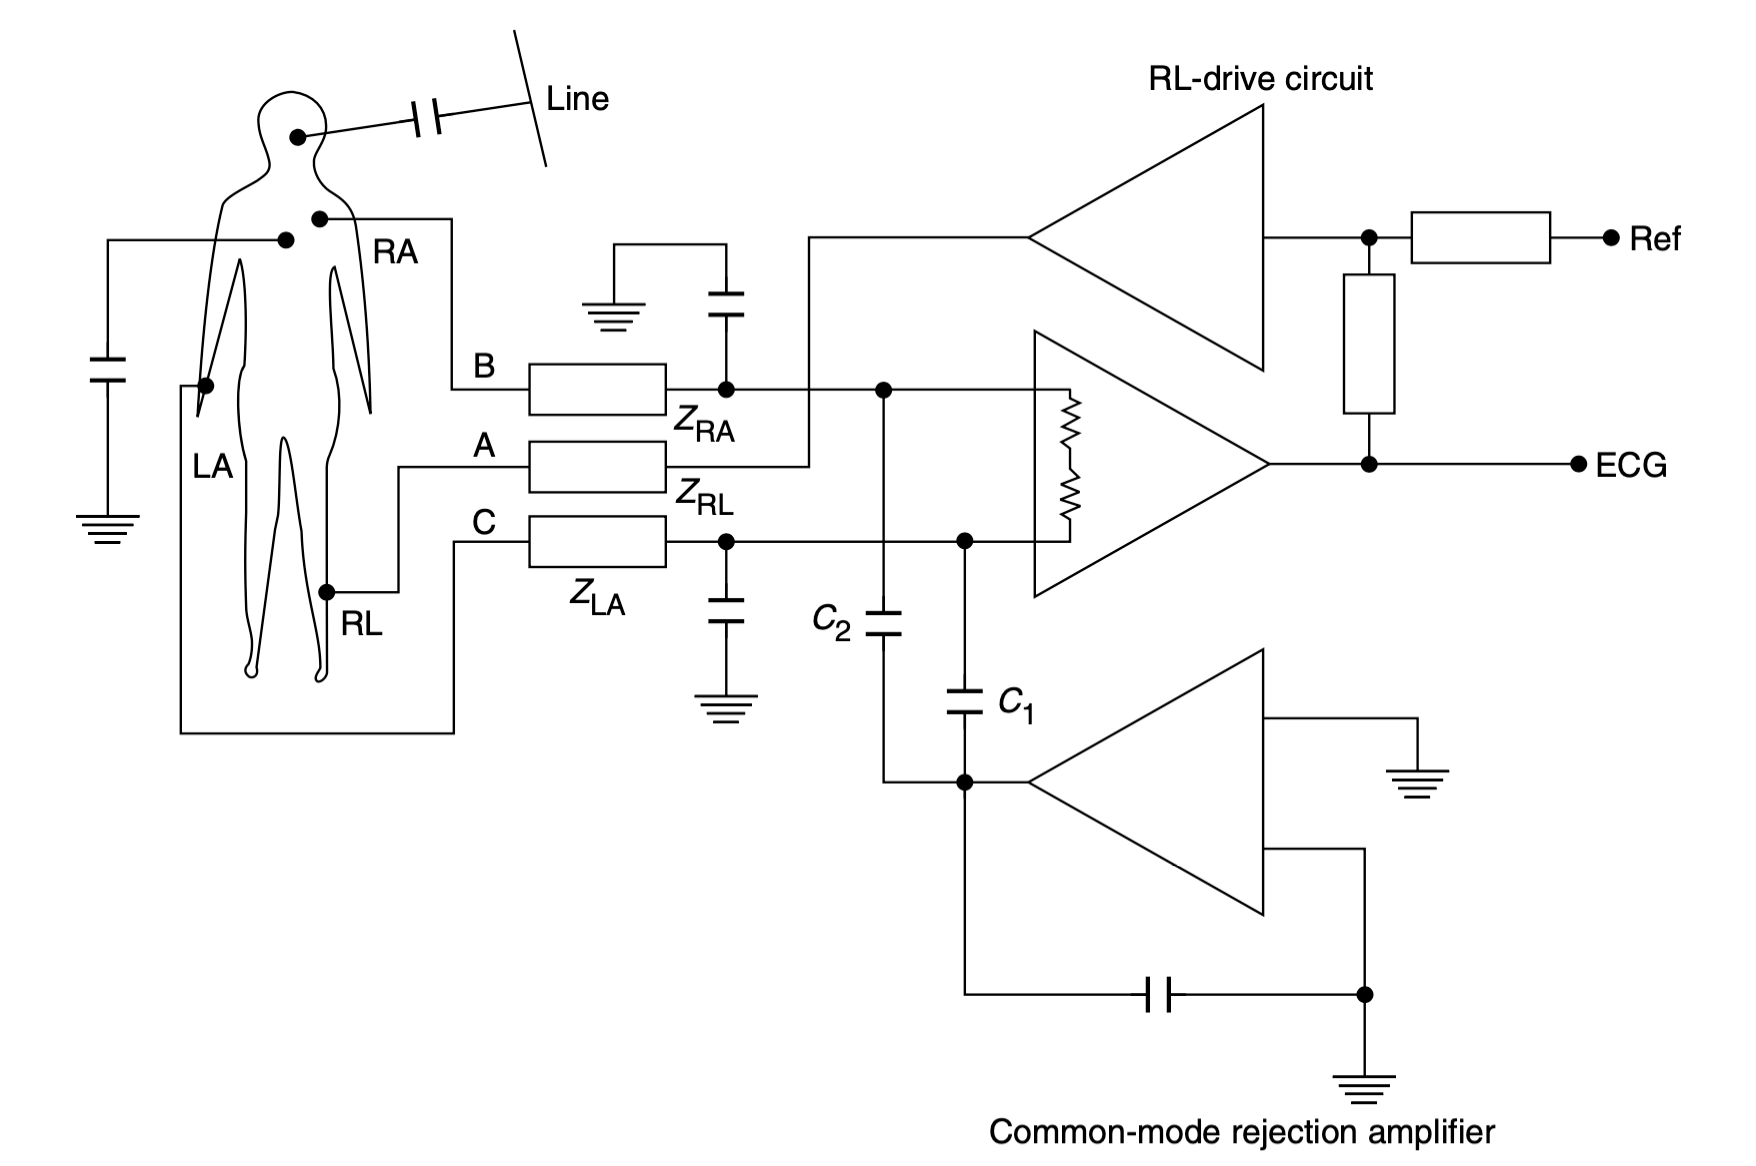
\includegraphics[scale=0.4]{Screenshot 2023-05-02 at 7.36.40 PM.png}
\end{center}
\section{Analysis of the ECG leads}
Two electrodes placed over different areas of the heart and connected to the galvanometer will pick up the electrical currents resulting from the potential difference between them. The resulting tracing of voltage difference at any two sites due to electrical activity of the heart is called a "LEAD".\\
\subsection{Bipolar leads}
In bipolar leads, ECG is recorded by using two electrodes such that the final trace corresponds to the difference of electrical potentials existing between them. They are called standard leads and have been universally adopted.\\
\\
In standard lead I, the electrodes are placed on the right and the left arm (RA and LA). In lead II, the electrodes are placed on the right arm and the left leg and in lead Ill, they are placed on the left arm and the left leg.\\
\\
In all lead connections, the difference of potential measured between two electrodes is always with reference to a third point on the body. This reference point is conventionally taken as the “right leg”.\\
The electric field of the heart could be represented diagrammatically as a triangle, with the heart ideally located at the centre. The triangle, known as the “Einthoven triangle”. It was shown that the instantaneous voltage measured from any one of the three limb lead positions is approximately equal to the algebraic sum of the other two or that the vector sum of the projections on all three lines is equal to zero.
\begin{center}
    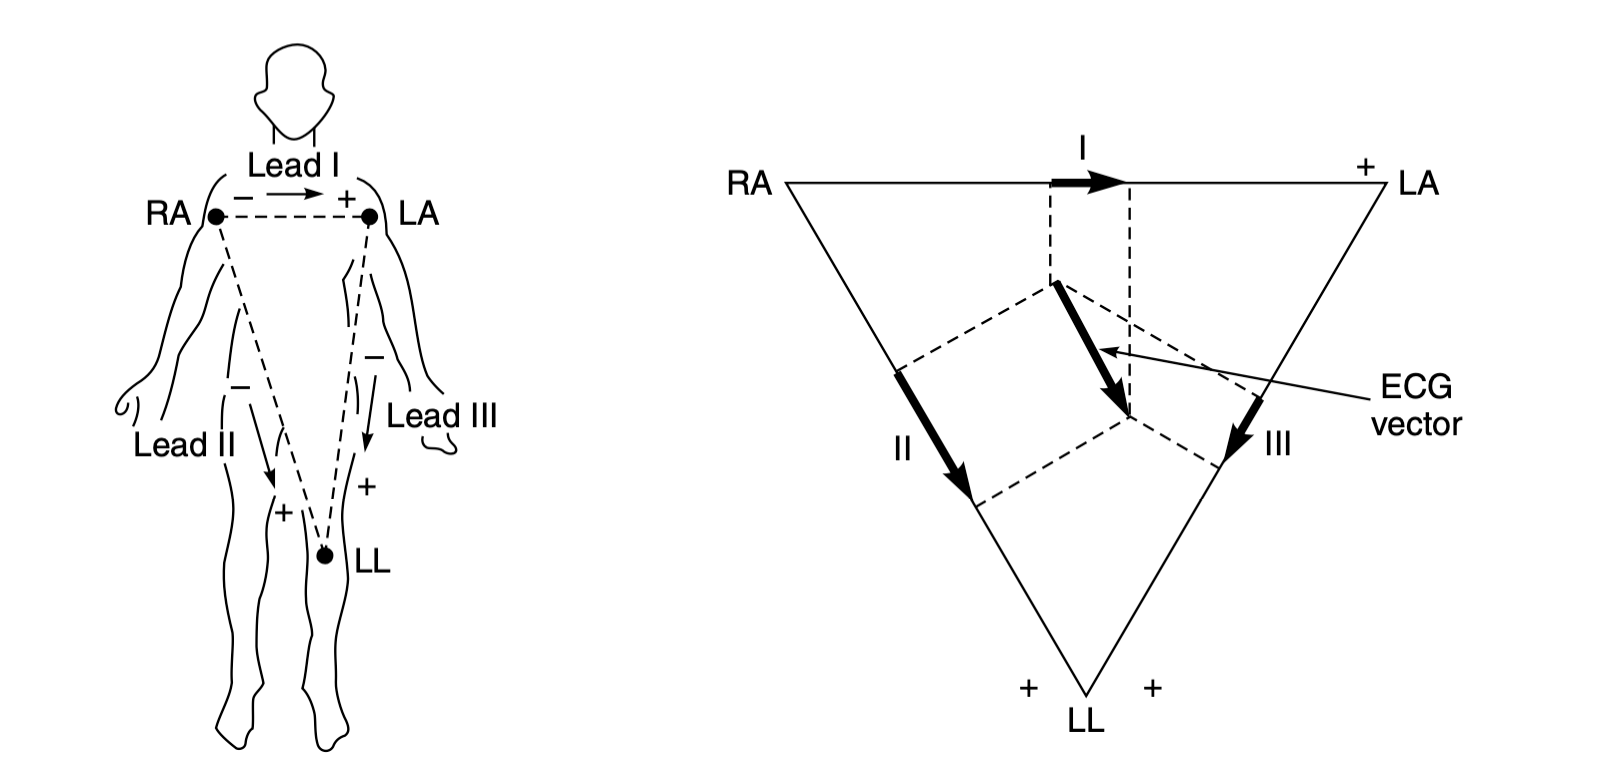
\includegraphics[scale=0.4]{Screenshot 2023-05-03 at 1.11.19 AM.png}
\end{center}
\subsection{Unipolar Leads (V Leads)}
There is quite often a smaller change witnessed in either of the potentials so it was proposed that better sensitivity can be obtained if we use a single electrode. If the electrode is placed closer to the heart, higher potentials will be observed. This lead to the development of unipolar leads introduced by Wilson in 1894. In this arrangement, the electrocardiogram is recorded between a single exploratory electrode and the central terminal, which has a potential corresponding to the centre of the body. In practice, the reference electrode or central terminal is obtained by a combination of several electrodes tied together at one point. 
\subsubsection{Limb Leads}
In this type of measurements, two limbs are tied together and recorded with respect to the third limb. In the limb identified as AVR, the right arm is recorded with respect to a reference established by joining the left arm and left leg electrodes.\\
They are also called augmented leads or ‘averaging leads’. The resistances inserted between the electrodes-machine connections are known as ‘averaging resistances’.
\subsubsection{Precordial Leads}
It employs an exploring electrode to record the potential of the heart action on the chest at six different positions. These leads are designated by the capital letter ‘V’ followed by a subscript numeral, which represents the position of the electrode on the pericardium. 
\begin{center}
    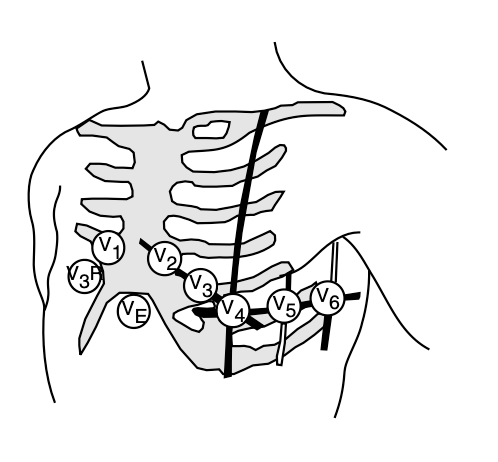
\includegraphics[scale=0.4]{Screenshot 2023-05-03 at 1.24.33 PM.png}
\end{center}
\section{Effect of Artefacts on ECG Recordings}
\subsection{Interference from the Power Line}
Power line interference is very easily identifiable as the ECG has a frequency of 50Hz. This interference may be due to the stray effect of the alternating current on the patient or because of alternating current effects of the wireloops in the patient cable. Another possible cause could be the loose connection of the wire and dirty electrodes.\\
The most common cause of the 50Hz interference is the disconnected electrode resulting in a very strong disturbing signal. It is sometimes strong enough to obliterate the stylus of the ECG machine and hence needs quick attention.\\
Electromagnetic interference from the power lines also results in poor quality tracings. Electrical equipment such as air-conditioners, elevators and X-ray units draw heavy power-line current, which induce 50 Hz signals in the input circuits of ECG machines. Due to unbalanced linkages, common mode rejection circuits almost prove ineffective against them.
\subsection{Shifting of the baseline}
A wandering baseline but otherwise normal ECG trace is usually due to the movement of the patient or electrodes. The baseline shift can be eliminated by ensuring that the patient lies relaxed and the electrodes are properly attached. 
\subsection{Muscle Tremor}
An irregular trembling of the ECG wave occurs, without wandering off the baseline in case the patient is not relaxed or cold. Muscle tremor signals are especially bothersome on limb leads when a patient moves or the muscles are stretched. 
\section{Two Types of ECG Machines}
\subsection{Microprocessor based ECG Machines}
Microprocessor technology has been employed in the electrocardiographs to attain certain desirable features like removal of artefacts, baseline wander, etc. using software techniques. Automatic centering of the tracing is another feature which can be similarly achieved.\\
\\
Microprocessor-based ECG machines can perform self-testing each time they are switched on. These machines are programmed to check lead continuity and polarity and also indicate lead fall- off or reversal. Use of digital filters considerably improves signal quality during recording and problems like baseline drift and excessive mains hum are thus automatically corrected. For this, the programs are stored in EPROM to obtain good quality tracings. Minimising baseline drift without distorting the signal helps in monitoring the ECG of exercising or ambulatory subjects.
\subsection{Multi-channel ECG Machine}
They carry several amplifier channels and a corresponding number of recording pens. This facilitates recording of several ECG leads simultaneously and thus considerably reduces the time required to complete a set of recordings. Another advantage of multi-channel recording is that the waveforms are recorded simultaneously and they can be shown in their proper time relationship with respect to each other.
\section{Holter's Test}
A Holter monitor is a small, wearable device that records the heart's rhythm. It's used to detect or determine the risk of irregular heartbeats (arrhythmias).
\\
A Holter monitor test may be done if a traditional electrocardiogram (ECG or EKG) doesn't provide enough details about the heart's condition. If the irregular heartbeats are infrequent, a longer term monitor called an event recorder may be needed.
\end{document}
